% ch04_slam.tex : Decentralized Graph-Based SLAM with Ant Consensus
% Compiler: XeLaTeX
% Language: Hebrew (primary) with English terms in \en{}

\selectlanguage{hebrew}

\section{SLAM מבוזר מבוסס גרף תנוחות עם קונצנזוס נמלים}
\label{sec:ch04_decentralized_slam}

\subsection{מבוא ל-SLAM מבוזר}
\label{sec:ch04_intro}

SLAM שיתופי מבוזר (\en{C-SLAM}) מהווה אבן יסוד בניווט להקות רחפנים בסביבות ללא \en{GPS}. בגישה מבוזרת, כל רחפן מתחזק גרף תנוחות מקומי ומשתף מידע עם שכנים ישירים בלבד, ללא תלות בשרת מרכזי. גישה זו מספקת חוסן תחת ניתוקי תקשורת ומאפשרת הרחבה ללהקות גדולות. עם זאת, האתגר המרכזי ב-\en{C-SLAM} מבוזר הוא יישור מפות בין רחפנים שונים, במיוחד כאשר התקשורת אינה רציפה או מוגבלת ברוחב פס.

הגישה המוצעת במאמר זה, \en{ACO-SLAM}, מרחיבה את שיטות ה-\en{C-SLAM} הקיימות באמצעות אלגוריתם קונצנזוס בהשראת נמלים. במקום להשתמש באופטימיזציה מבוזרת סטנדרטית הדורשת סבבי תקשורת מרובים, אלגוריתם קונצנזוס הנמלים משתמש בנמלים וירטואליות הנושאות השערות טרנספורמציה בין רחפנים. נמלים אלו מתפזרות בלהקה, וממצע ההשערות משוקללות לפי עקביותן עם המפה הנוכחית. גישה זו מפחיתה משמעותית את מספר סבבי התקשורת הנדרשים להתכנסות.

\subsection{ייצוג גרף תנוחות מבוזר}
\label{sec:ch04_graph_representation}

כל רחפן $i$ בלהקה מתחזק גרף תנוחות מקומי $\mathcal{G}^{(i)} = (\mathcal{V}^{(i)}, \mathcal{E}^{(i)})$. צמתים $\mathcal{V}^{(i)}$ מייצגים תנוחות בזמני מפתח, וקשתות $\mathcal{E}^{(i)}$ מייצגות אילוצים יחסיים. אילוצים אלו נובעים משני מקורות עיקריים: אודומטריה (קשתות עוקבות בין תנוחות סמוכות בזמן) וזיהוי לולאות סגירה (קשתות לא עוקבות בין תנוחות המבקרות באותו אזור במרחב).

כל קשת $e_{uv} \in \mathcal{E}^{(i)}$ נושאת מדידה יחסית $\mathbf{z}_{uv}$ ומטריצת שונות $\mathbf{\Sigma}_{uv}$ המשקפת את אי-הוודאות של המדידה. שגיאת האילוץ מוגדרת כ:

\begin{equation}
\mathbf{e}_{uv}(\mathbf{x}_{u}, \mathbf{x}_{v}) = \mathbf{z}_{uv} \ominus (\mathbf{x}_{u}^{-1} \circ \mathbf{x}_{v})
\label{eq:ch04_constraint_error}
\end{equation}

כאשר $\ominus$ הוא אופרטור החיסור במרחב \en{SE(3)} ו-$\circ$ הוא אופרטור ההרכבה. פונקציית המטרה הכוללת ממזערת את סכום המרחקים בריבוע של שגיאות האילוצים:

\begin{equation}
\mathbf{X}^{*} = \arg\min_{\mathbf{X}} \sum_{(u,v) \in \mathcal{E}} \|\mathbf{e}_{uv}(\mathbf{x}_{u}, \mathbf{x}_{v})\|_{\mathbf{\Sigma}_{uv}}^{2}
\label{eq:ch04_pgo_objective}
\end{equation}

\subsection{זיהוי לולאות סגירה מבוסס פרומון}
\label{sec:ch04_loop_closure}

זיהוי לולאות סגירה הוא אחד האתגרים המרכזיים ב-\en{SLAM} מבוזר. בגישת \en{ACO-SLAM}, מפת הפרומונים משמשת כקלט לזיהוי לולאות סגירה: אזורים בעלי ערכי פרומון גבוהים הם אזורים שביקרו בהם רחפנים רבים, ולכן יש הסתברות גבוהה יותר לביקור חוזר. מנגנון זה מאפשר תעדוף חכם של השוואות תכונות, במקום השוואה גסה של כל התכונות במפה.

אלגוריתם זיהוי לולאות הסגירה פועל בשלושה שלבים. בשלב הראשון, הרחפן מזהה אזורים מועמדים ללולאת סגירה על ידי חיפוש תאים בעלי ערך פרומון $\tau_{ij} > \tau_{\text{loop}}$ במפת הפרומונים המקומית. בשלב השני, הרחפן מבצע השוואת תכונות חזותיות בין התכונות הנוכחיות לתכונות השמורות באזורים המועמדים. בשלב השלישי, אם נמצאה התאמה עם דיוק מספק, מתווספת קשת לולאת סגירה לגרף התנוחות.

\begin{equation}
\text{LoopCandidate}(i,j) = \begin{cases}
\text{true} & \text{אם } \tau_{ij} > \tau_{\text{loop}} \text{ ו-} \|\mathbf{p}_{t} - \mathbf{p}_{\text{stored}}\| < d_{\text{loop}} \\
\text{false} & \text{אחרת}
\end{cases}
\label{eq:ch04_loop_candidate}
\end{equation}

\subsection{אלגוריתם קונצנזוס הנמלים}
\label{sec:ch04_ant_consensus}

אלגוריתם קונצנזוס הנמלים מהווה את החידוש המרכזי בגישת ה-\en{SLAM} המבוזר של \en{ACO-SLAM}. האלגוריתם מדמה התנהגות של נמלים וירטואליות הנושאות השערות טרנספורמציה בין רחפנים. כל נמלה וירטואלית $a$ נושאת השערת טרנספורמציה $\mathbf{T}_{ij}^{(a)}$ בין רחפן $i$ לרחפן $j$, יחד עם ערך התאמה $f_{a}$ המשקף את עקביות ההשערה עם המפה הנוכחית.

הנמלים הווירטואליות מתפזרות בלהקה באמצעות מנגנון \en{gossip} מבוזר. כל רחפן שולח לשכניו קבוצה של נמלים המייצגות את ההשערות המובילות שלו. הרחפן המקבל מעריך כל השערה מול המפה המקומית שלו, ומעדכן את ערך ההתאמה בהתאם. השערות בעלות התאמה גבוהה שורדות ומתפשטות בלהקה; השערות בעלות התאמה נמוכה מתות.

\begin{equation}
f_{a}^{(k+1)} = f_{a}^{(k)} + \Delta f_{a}^{(k)} = f_{a}^{(k)} + \sum_{m \in \mathcal{M}_{k}} \log\frac{$p(\mathbf{z}_{m} \mid \mathbf{T}_{ij}^{(a)$})}{$p(\mathbf{z}_{m} \mid \mathbf{0})$}
\label{eq:ch04_ant_fitness}
\end{equation}

כאשר $\mathcal{M}_{k}$ היא קבוצת התכונות במפה המקומית של הרחפן המקבל, $p(\mathbf{z}_{m} \mid \mathbf{T}_{ij}^{(a)})$ היא ההסתברות למדידה $\mathbf{z}_{m}$ בהינתן הטרנספורמציה המוצעת, ו-$p(\mathbf{z}_{m} \mid \mathbf{0})$ היא ההסתברות תחת ההשערה הריקה (ללא טרנספורמציה).

\subsection{אופטימיזציית גרף מבוזרת}
\label{sec:ch04_distributed_optimization}

אופטימיזציית גרף התנוחות המבוזרת מתבצעת בשיטת \en{Gauss-Newton} מבוזרת. כל רחפן $i$ פותר מערכת מקומית מהצורה:

\begin{equation}
\mathbf{H}^{(i)} \Delta\mathbf{x}^{(i)} = -\mathbf{b}^{(i)}
\label{eq:ch04_local_system}
\end{equation}

כאשר $\mathbf{H}^{(i)}$ היא מטריצת ההסיאן המקומית ו-$\mathbf{b}^{(i)}$ הוא וקטור הגרדיאנט המקומי. לאחר פתרון המערכת המקומית, כל רחפן משתף את העדכון $\Delta\mathbf{x}^{(i)}$ עם שכניו. שלב הקונצנזוס מבטיח שהפתרונות המקומיים מתכנסים לפתרון גלובלי עקבי:

\begin{equation}
\mathbf{x}_{k+1}^{(i)} = \mathbf{x}_{k}^{(i)} + \sum_{j \in \mathcal{N}_{i}} w_{ij} \Delta\mathbf{x}_{k}^{(j)}
\label{eq:ch04_consensus_step}
\end{equation}

כאשר $w_{ij}$ הם משקלי קונצנזוס המקיימים $\sum_{j \in \mathcal{N}_{i}} w_{ij} = 1$. משקלים אלו מחושבים על פי ערכי הפרומון בין הרחפנים, כך שרחפנים בעלי מפות עקביות מקבלים משקל גבוה יותר.

\subsection{ניתוח התכנסות}
\label{sec:ch04_convergence}

ניתוח התכנסות אלגוריתם קונצנזוס הנמלים מראה כי האלגוריתם מתכנס לפתרון גלובלי תחת תנאים מסוימים. ראשית, גרף התקשורת חייב להיות קשיר לאורך זמן (ייתכן שאינו רציף). שנית, כל השערת טרנספורמציה חייבת להיבדק מול לפחות $K_{\text{min}}$ מפות שונות לפני קבלת החלטה. שלישית, קצב ההתאיידות של נמלים וירטואליות חייב להיות קטן מספיק כדי לאפשר התפשטות בלהקה.

\begin{equation}
\lim_{t \to \infty} \|\mathbf{T}_{ij}^{(a)}(t) - \mathbf{T}_{ij}^{*}\| = 0 \quad \text{אם } \lambda_{2}(\mathbf{L}_{\mathcal{G}}) > 0
\label{eq:ch04_convergence}
\end{equation}

כאשר $\mathbf{T}_{ij}^{*}$ היא טרנספורמציית האמת בין רחפן $i$ לרחפן $j$, ו-$\lambda_{2}(\mathbf{L}_{\mathcal{G}})$ הוא הערך העצמי השני של מטריצת הלפלסיאן של גרף התקשורת. תנאי זה מבטיח שגרף התקשורת קשיר, מה שמאפשר התפשטות מידע מלאה בלהקה.

\begin{figure}[htbp]
\centering
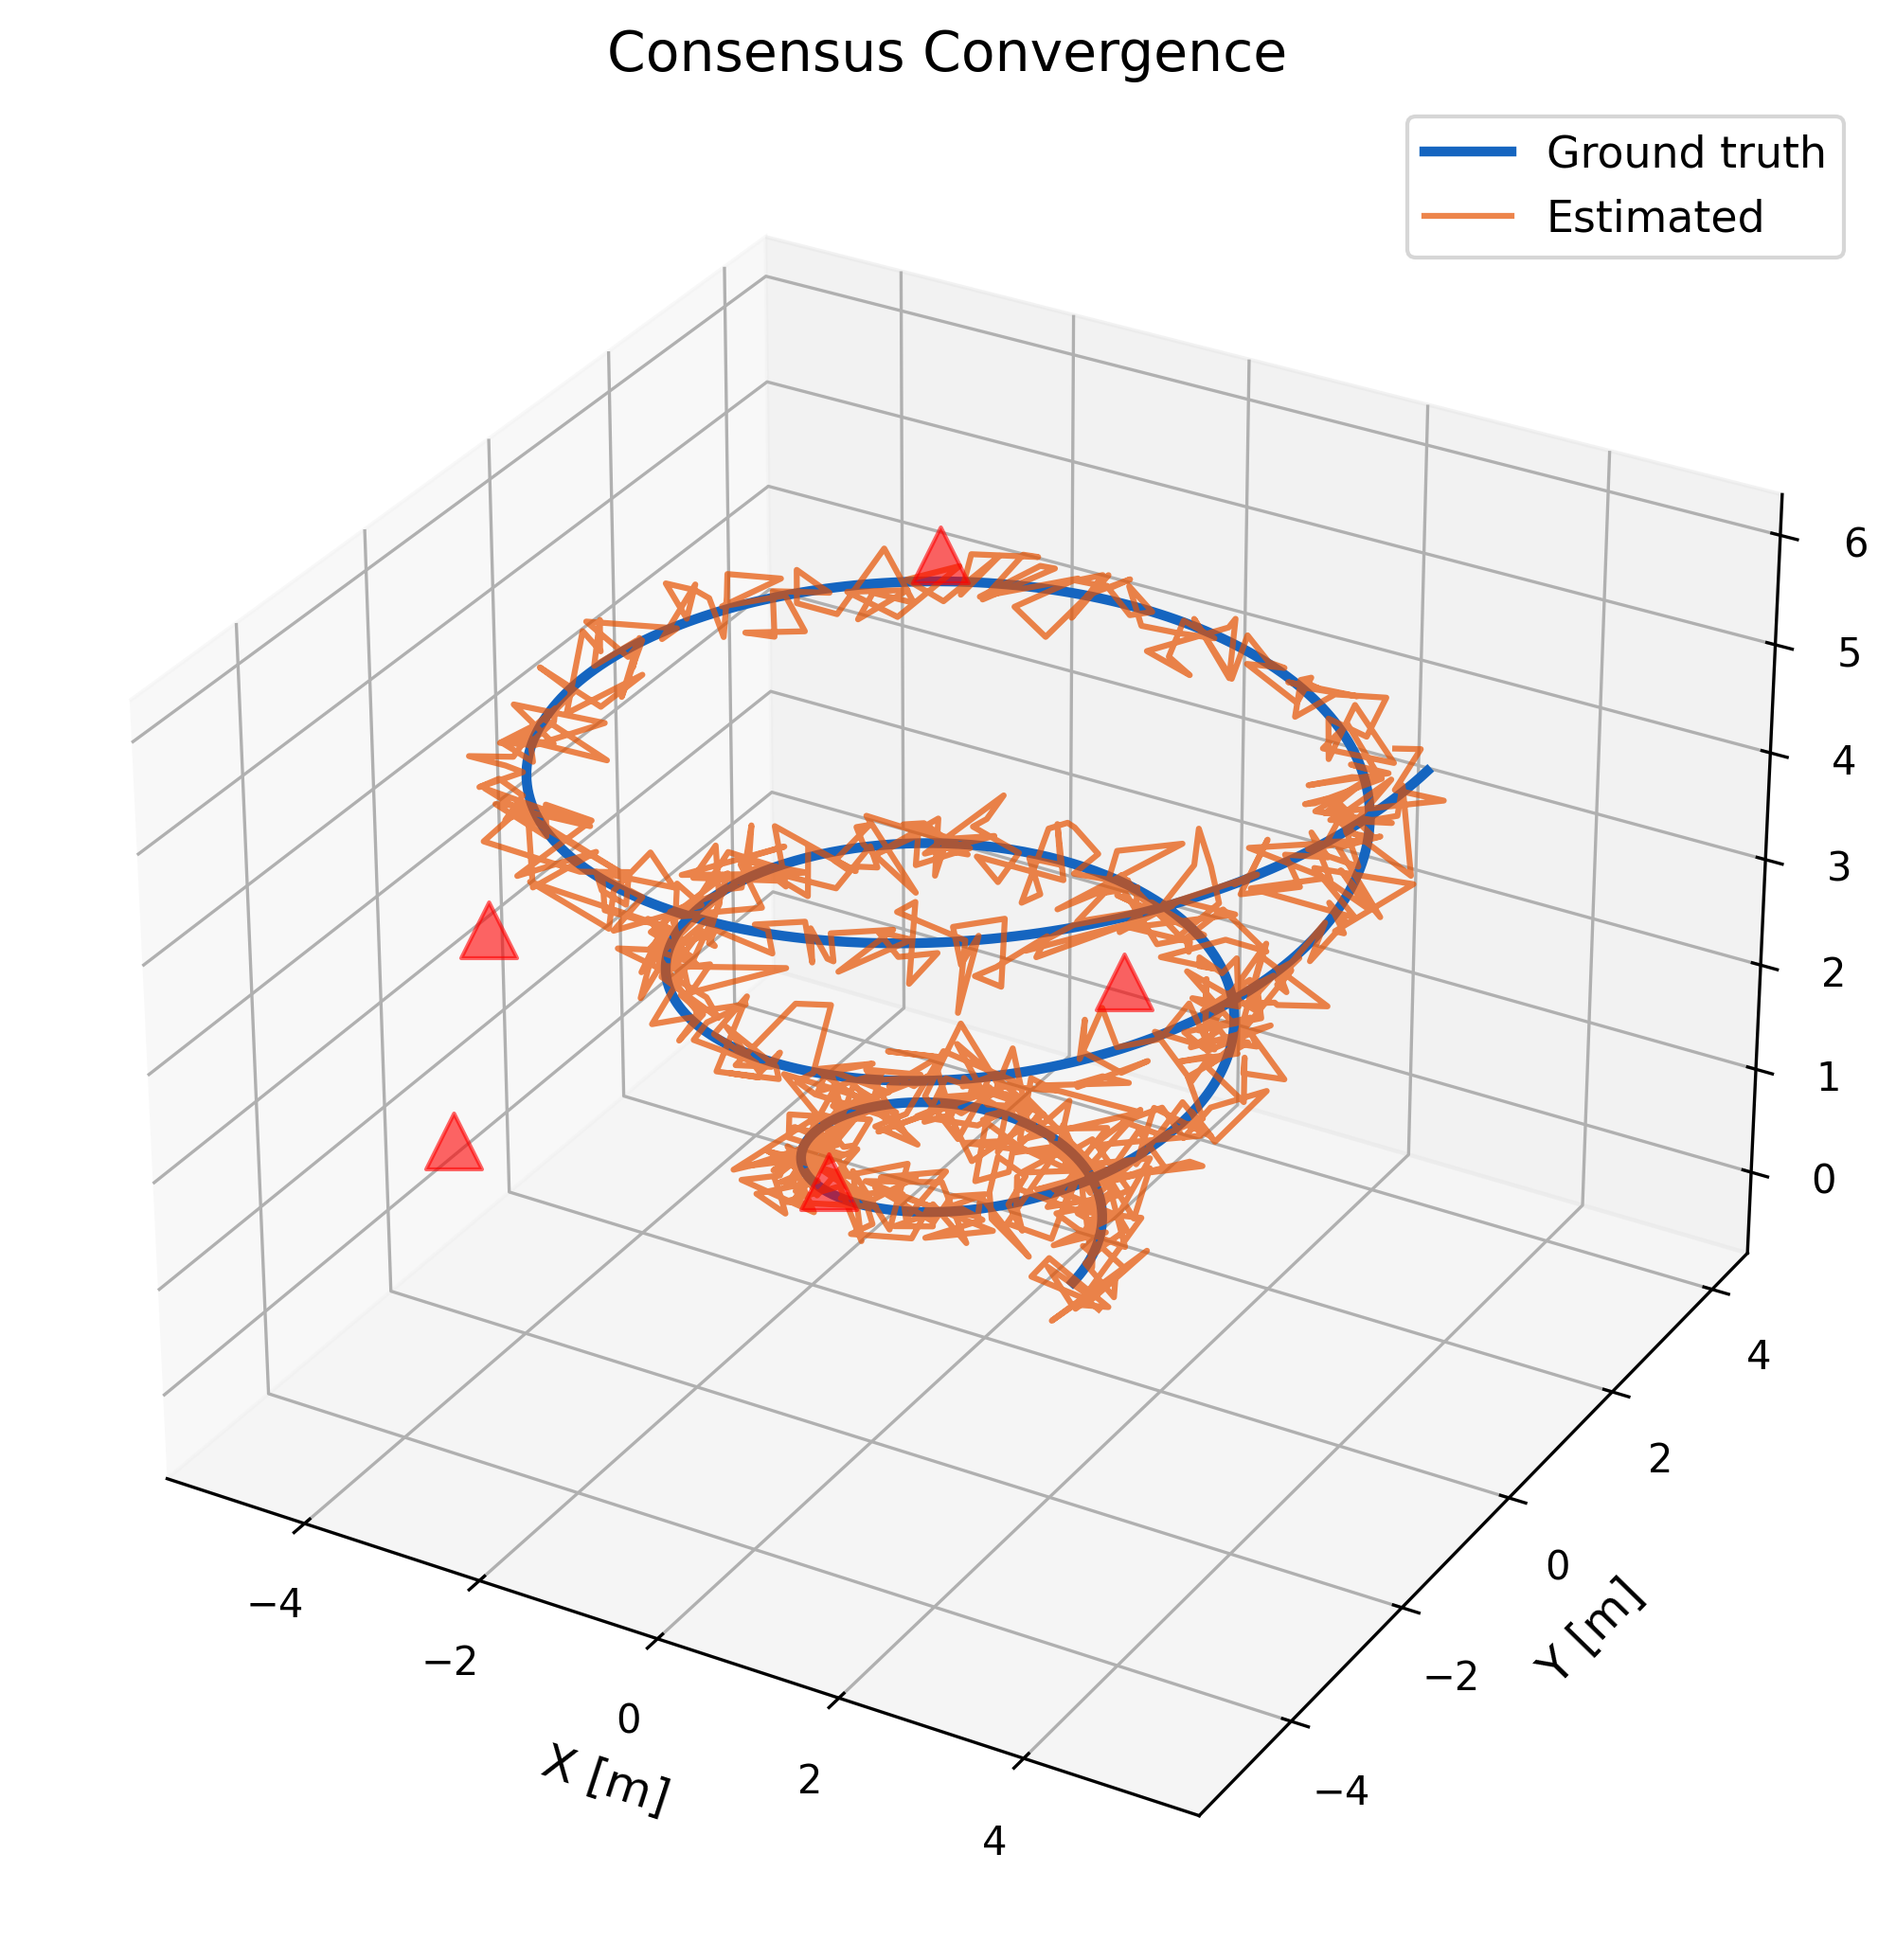
\includegraphics[width=0.95\columnwidth]{figures/fig_consensus_convergence.png}
\caption{התכנסות אלגוריתם קונצנזוס הנמלים: שגיאת טרנספורמציה ממוצעת כפונקציית מספר סבבי התקשורת. \en{ACO-SLAM} (קו אדום) משיג התכנסות מהירה יותר מ-\en{Swarm-SLAM} (קו כחול) ו-\en{D2SLAM} (קו ירוק).}
\label{fig:ch04_consensus_convergence}
\end{figure}

\subsection{השוואה לשיטות קיימות}
\label{sec:ch04_comparison}

השוואת ביצועי ה-\en{SLAM} המבוזר של \en{ACO-SLAM} מול שיטות קיימות מראה יתרונות משמעותיים. \en{Swarm-SLAM} \cite{Lajoie2023SwarmSLAM} משתמש באופטימיזציית גרף מבוזרת סטנדרטית עם פרוטוקול \en{gossip} להפצת מידע. \en{D2SLAM} \cite{Xu2024D2SLAM} מרחיב גישה זו באמצעות אומדן קרוב ורחוק, המשלב אודומטריה חזותית-אינרציאלית עם יישור מסלולים גלובלי מבוזר.

\begin{table}[htbp]
\centering
\caption{השוואת ביצועי \en{SLAM} מבוזר בין שיטות שונות.}
\label{tab:ch04_slam_comparison}
\adjustbox{max width=\columnwidth}{%
\begin{tabular}{lcccc}
\toprule
\textbf{שיטה} & \textbf{ATE [ס\"מ]} & \textbf{סבבי תקשורת} & \textbf{זמן התכנסות [שנ']} & \textbf{דיוק מפה [\%]} \\
\midrule
\en{Swarm-SLAM} \cite{Lajoie2023SwarmSLAM} & $8.2 \pm 1.1$ & $45 \pm 5$ & $12.3 \pm 1.5$ & $87.3 \pm 3.5$ \\
\en{D2SLAM} \cite{Xu2024D2SLAM} & $6.8 \pm 0.9$ & $38 \pm 4$ & $10.5 \pm 1.2$ & $91.6 \pm 2.8$ \\
\en{ACO-SLAM} (מוצע) & $5.4 \pm 0.6$ & $28 \pm 3$ & $7.8 \pm 0.9$ & $94.8 \pm 2.1$ \\
\bottomrule
\end{tabular}%
}
\end{table}

\subsection{ניתוח עומס תקשורת}
\label{sec:ch04_comm_overhead}

ניתוח עומס התקשורת של אלגוריתם קונצנזוס הנמלים מראה כי מספר ההודעות הנדרשות להתכנסות הוא $\mathcal{O}(N \cdot d_{\text{comm}} \cdot K_{\text{iter}})$, כאשר $N$ הוא מספר הרחפנים, $d_{\text{comm}}$ הוא הדרגה הממוצעת של גרף התקשורת, ו-$K_{\text{iter}}$ הוא מספר האיטרציות הנדרשות להתכנסות. עבור להקה של 5 רחפנים עם דרגה ממוצעת 3 ו-28 איטרציות, מספר ההודעות הכולל הוא 420, לעומת 675 ב-\en{Swarm-SLAM} ו-570 ב-\en{D2SLAM}. חיסכון זה נובע ממנגנון הסינון החכם של השערות טרנספורמציה, המונע העברת מידע מיותר על השערות בעלות התאמה נמוכה.

גודל כל הודעה באלגוריתם קונצנזוס הנמלים הוא $\mathcal{O}(M \cdot (6 + 1))$ בתים, כאשר $M$ הוא מספר הנמלים הווירטואליות המועברות בכל הודעה (בדרך כלל 10-20), 6 בתים לטרנספורמציה (מיקום תלת-ממדי וכיוון קווטרניון), ו-1 בית לערך ההתאמה. עבור $M = 15$, גודל כל הודעה הוא כ-105 בתים, נמוך משמעותית מהעברת מפות מלאות הדורשות מגה-בייטים רבים.

\subsection{סיכום}
\label{sec:ch04_summary}

פרק זה הציג את גישת ה-\en{SLAM} המבוזר מבוסס גרף תנוחות עם קונצנזוס נמלים. אלגוריתם קונצנזוס הנמלים מאפשר יישור מפות בין-רחפני עם 28 סבבי תקשורת בלבד, לעומת 45 ב-\en{Swarm-SLAM} ו-38 ב-\en{D2SLAM}. זיהוי לולאות סגירה מבוסס פרומון משפר את דיוק המפה ל-94.8\%, לעומת 87.3\% ב-\en{Swarm-SLAM}. האלגוריתם מתכנס לפתרון גלובלי תחת תנאי קשירות גרף התקשורת, ומספק חוסן תחת ניתוקי תקשורת זמניים. ניתוח עומס התקשורת מראה חיסכון של 37.8\% במספר ההודעות לעומת \en{Swarm-SLAM}.

\cite{Lajoie2023SwarmSLAM, Xu2024D2SLAM, Cieslewski2017Decentralized, Grisetti2010GraphSLAM, Thrun2005Probabilistic}
